\section{Introduction}

\subsection{LSST Data Management System}

To carry out this mission the Data Management System (DMS) performs the following major functions:

\begin{itemize}
\item Processes the incoming stream of images generated by the camera
  system during observing to produce transient alerts and to archive
  the raw images.

\item Roughly once per year, creates and archives a Data Release (``DR''),
  which is a static self-consistent collection of data products
  generated from all survey data taken from the date of survey
  initiation to the cutoff date for the Data Release. The data
  products (described in detail in the \DPDD), include measurements of 
  the properties (shapes, positions, fluxes, motions, etc.) of all detected
  objects, including those below the single visit sensitivity limit,
  astrometric and photometric calibration of the full survey object
  catalog, and limited classification of objects based on both their
  static properties and time-dependent behavior.  Deep coadded images
  of the full survey area are produced as well.

\item Periodically creates new calibration data products, such as bias
  frames and flat fields, that will be used by the other processing
  functions, as necessary to enable the creation of the data products above.

\item Makes all LSST data available through interfaces that utilize,
  to the maximum possible extent, community-based standards such as those
  being developed by the Virtual Observatory (``VO''), and facilitates user
  data analysis and the production of user-defined data products at Data
  Access Centers (``DAC'') and at external sites.
\end{itemize}

The overall architecture of the DMS is discussed in more detail in the Data Management System Design (\DMSD) document. The overall architecture of the DMS is shown in Figure~\ref{fig:DMS}.
\\

This document discusses the role of the Applications layer in the first three functions listed above (the functions involving \emph{science pipelines}).  The fourth is discussed separately in the SUI Conceptual Design Document (\SUI).

\begin{figure}
\centering
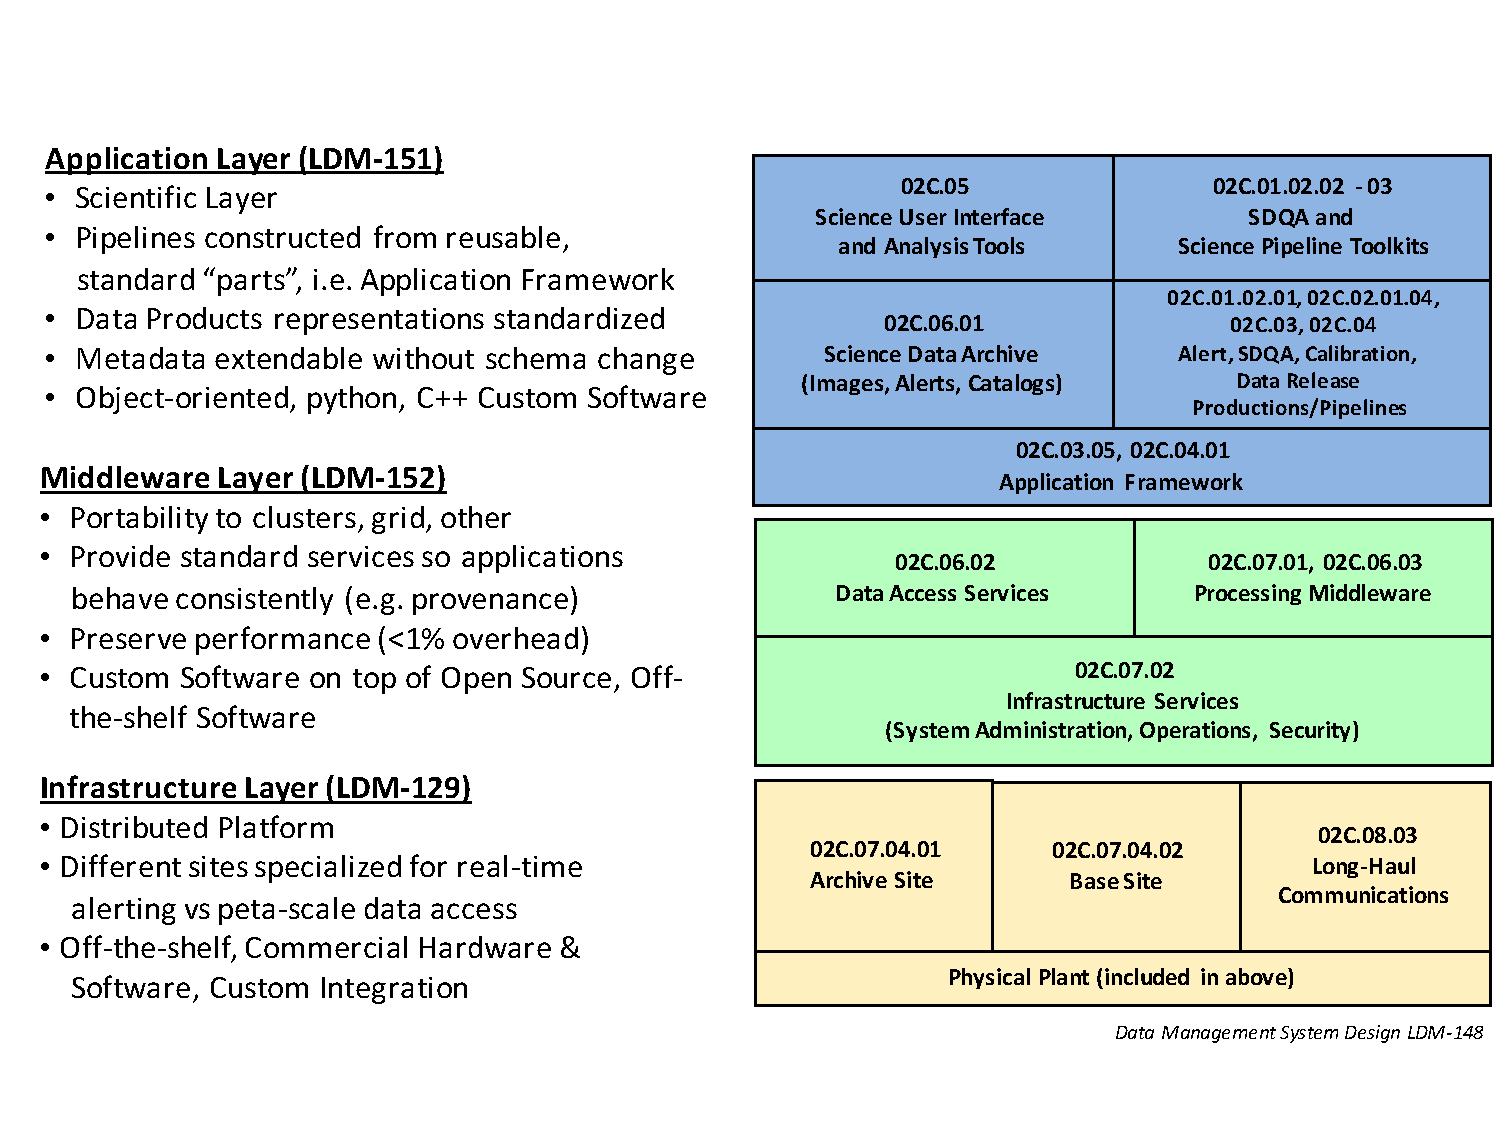
\includegraphics[angle=90,scale=0.70]{figures/DMS-Architecture.pdf}
\caption{Architecture of the Data Management System\label{fig:DMS}}
\end{figure}

\begin{figure}
%\includegraphics[angle=90,scale=0.70]{ApplicationLayerProductionsandPipelines.eps}
\centering
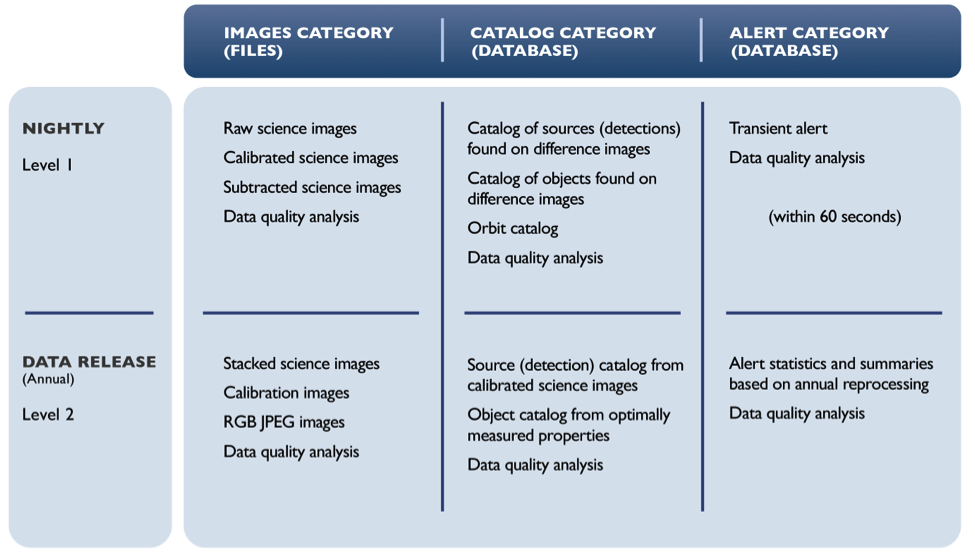
\includegraphics[angle=90]{figures/DataProductDelivarables.png}
\caption{Organization of LSST Data Products\label{fig:DP}}
\end{figure}

\subsection{Data Products}

The LSST data products are organized into three groups, based on their intended use and/or origin. The full description is provided in the Data Products Definition Document (\DPDD); we summarize the key properties here to provide the necessary context for the discussion to follow. 

\begin{itemize}
\item {\bf Level 1} products are intended to support timely detection and follow-up
  of time-domain events (variable and transient sources). They are generated by
  near-real-time processing the stream of data from the camera system during 
  normal observing.  Level 1 products are therefore continuously generated and / or
  updated every observing night. This process is of necessity highly
  automated, and must proceed with absolutely minimal human
  interaction.  In addition to science data products, a number of related
  Level 1 ``SDQA''\footnote{Science Data Quality Analysis} data products are generated
  to assess quality and to provide feedback to the Observatory Control System (OCS).

\item {\bf Level 2} products are generated as part of a Data Release, generally
  performed 
  yearly, with an additional data release for the first 6 months of survey data. 
  Level 2 includes data products for which extensive
  computation is required, often because they combine information from
  many exposures.  Although the steps that generate Level 2 products
  will be automated, significant human interaction may be required at
  key points to ensure the quality of the data.

\item {\bf Level 3} products are generated on any computing resources
  anywhere and then stored in an LSST Data Access Center. Often, but not
  necessarily, they will be generated by users of LSST using LSST software
  and/or hardware. LSST DM is required to facilitate the creation of
  Level 3 data products by providing suitable APIs, software components, and
  computing infrastructure, but will not by itself create any Level 3
  data products. Once created, Level 3 data products may be associated with
  Level 1 and Level 2 data products through database federation.
  Where appropriate, the LSST Project, with the agreement of the Level 3
  creators, may incorporate user-contributed Level 3 data product pipelines
  into the DMS production flow, thereby promoting them to Level 1 or 2.

\end{itemize}
%
The organization of LSST Data Products is shown in Figure~\ref{fig:DP}.

Level 1 and Level 2 data products that have passed quality control
tests will be accessible to the public without restriction.
Additionally, the source code used to generate them will be made
available, and LSST will provide support for builds on selected
platforms.

\subsection{Science Pipelines Overview}

We recognize four major groups of science pipelines residing in the Applications layer:
\begin{itemize}
    \item {\bf Level 1 Pipelines}, grouped under the {\bf Alert Production} element of the WBS, are designed to generate Level 1 data products. These include:
    \begin{itemize}
    \item {\bf \emph{Single Frame Processing (``SFM'') Pipeline}} (\wbsSFM), to reduce acquired visits and detect and characterize astrophysical sources present in these visits.
    \item {\bf \emph{Image Differencing Pipeline}} (\wbsDiffim), to create difference images, and detect and characterize sources in them.
    \item {\bf \emph{Association Pipeline}} (\wbsAssocP), to associate sources detected in the difference images with known objects.
    \item {\bf \emph{Alert Generation Pipeline}} (\wbsAP), to generate and transmit alerts to time-domain events (e.g., transients) to the astronomical community, and
    \item {\bf \emph{Moving Object Pipeline}} (\wbsMOPS), to identify, link and compute orbits for Solar System objects detected in difference images.
    \end{itemize}
Level 1 pipelines run as the data are being acquired. They primarily focus on image differencing, and the reduction of information extracted from difference images. The algorithms they employ are designed and chosen to complete processing on minute (alert production) to day (\textbf{\emph{DayMOPS}}) time scales. They are also rerun as a part of Data Release Production (DRP), potentially in somewhat different configurations to achieve greater precision at the expense of increased runtime.
    
    \item {\bf Level 2 Pipelines} run annually or semi-annualy (for the first year of data), and are designed to generate deep co-adds and catalogs stemming from analysis of direct image data.  These include:
    \begin{itemize}
        \item {\bf \emph{PSF Estimation Pipeline}} (\wbsPSF), to estimate the PSF properties and variation across the focal plane for each visit, to the degree of precision required by the \SRD. Note that the work of this pipeline goes beyond the typical single-CCD PSF estimation present in the SFM pipeline.
        \item {\bf \emph{Image Coaddition Pipeline}} (\wbsCoadd), to generate and characterize coadded images of the sky, as well as create templates for image differencing.
        \item {\bf \emph{Object Detection and Deblending}} (\wbsDetDeblend), to detect sources in images of the sky and decompose them into individual astronomical objects.
        \item {\bf \emph{Object Characterization Pipeline}} (\wbsObjChar), to characterize (perform measurements of) astrophysical objects detected in LSST imaging (both in single frames and coadds).
    \end{itemize}
    
    \item {\bf Calibration Pipelines} process the collected calibration data and perform calibration of LSST instruments and data products. These include:
    \begin{itemize}
        \item {\bf \emph{Calibration Products Pipeline}} (\wbsCPP), that generates the necessary calibration data products (e.g., master flats, biases, atmospheric models, etc.). It is run periodically as new calibration data are acquired.
        \item {\bf \emph{Photometric Calibration Pipeline}} (\wbsPhotoCal), that performs global photometric self-calibration of the Level 2 dataset.
        \item {\bf \emph{Astrometric Calibration Pipeline}} (\wbsAstroCal), that performs global astrometric self-calibration of the Level 2 dataset.
    \end{itemize}
    The calibration products pipeline is also rerun as a part of Data Release Processing. Global self-calibration steps run in DRP only.

       \item {\bf Science Data Quality Assessment (SDQA) pipelines and toolkits}, to enable collection, computation, visualization, monitoring and analysis of data quality metrics across all pipelines. These are divided into:
       \begin{itemize}
           \item {\bf \emph{Science Data Quality Assessment Pipeline}} (\wbsSDQAP), that provides low-level data collection functionality for SDQA and
           \item {\bf \emph{Science Data Quality Analyst Toolkit}} (\wbsSDQAT), that provides the visualization, analysis and monitoring capabilities for SDQA.
       \end{itemize}

\end{itemize}

In addition to these four, we recognize two other, cross-cutting, elements of DMS functionality:

\begin{itemize}
       \item {\bf \emph{Common Image and Catalog Processing Framework}} (\wbsAFW), known as the {\bf Application Framework (afw)}, that collects base classes and algorithms % RHL need a better word than algorithms
         used by the DM Applications layer. The framework is split in two WBS elements, to reflect the multi-institutional nature of the work, but is functionally viewed as a single, integrated, component (class library).
       \item The {\bf \emph{Science Pipeline Toolkit}} (\wbsSPT), a collection of software components (and design principles) designed to enable construction of Level 3 pipelines relying on reusable lower-level components produced in support of other LSST DM software.
\end{itemize}

\subsubsection{Level 1 Pipelines Overview}
The production of Level 1 products is generally performed nightly, directly fed by 
the output data stream from the Camera SDS\footnote{Science Array Data Acquisition (DAQ) Subsystem} during observing. This data stream
contains both unprocessed (raw) camera images, and images that have been corrected
for crosstalk by the SDS on the Summit.  The normal observing
pattern is to take two 15 second exposures of the same field in immediate
succession.  These two exposures together form a {\em visit}, which is the typical
image data unit processed by the rest of the DM system.
\\

\begin{figure}
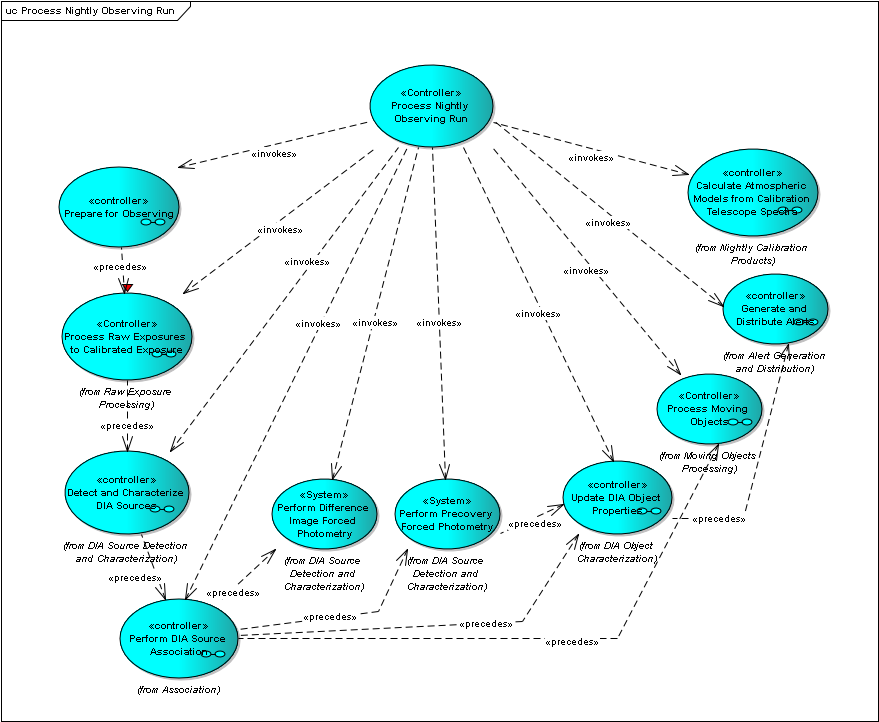
\includegraphics[angle=0,scale=0.44]{figures/process_nightly_observing_run.png}
\caption{Level 1 Processing Flow Diagram\label{fig:level1}}
\end{figure}

The logical flow of Level 1 processing is shown in the Use Case diagram presented in Figure~\ref{fig:level1}. For every observation, the following sequence of events will unfold:
%
\begin{enumerate}
\item A visit is acquired (\uc{Prepare for Observing}) and reduced (\uc{Process Raw Exposures to Calibrated Exposure}) to a single {\em visit image}. This includes instrumental signature removal\footnote{E.g., subtraction of bias and dark frames, flat fielding, bad pixel/column interpolation, etc.}, combining of snaps, etc.
  % RHL I removed cosmic ray rejection as it's not clear if it's in ISR or snap combination.

\item The visit image is differenced against the appropriate template and \DIASources are detected (\uc{Detect and Characterize DIA Sources}). If necessary, deblending is performed at this stage.

The flux and shape of the DIASource are measured on the difference image. PSF photometry is performed on the visit image at the position of the \DIASource to obtain a measure of the absolute flux.
  % RHL this is tricky in crowded fields (inc. SNe on galaxies).  We should rethink this a bit at some point.

\item The \DB is searched for a \DIAObject or an \SSObject with which to positionally associate the newly discovered \DIASource. If no match is found, a new \DIAObject is created and the observed \DIASource is associated to it.

If the \DIASource has been associated to an \SSObject (a known Solar System object), it will be flagged as such and an alert will be issued. Further processing will occur in daytime (\uc{Process Moving Objects}).

\item Otherwise, the associated \DIAObject measurements will be updated with new data (\uc{Update DIA Object Properties}). All affected columns will be recomputed, including proper motions, centroids, light curves, nearest Level 2 \Objects, etc.
  % RHL do we really want to update e.g. the proper motion/parallax on each visit?

\item An alert is issued (\uc{Generate and Distribute Alerts}) that includes all required components, as described in the \DPDD.

\item For all \DIAObjects overlapping the field of view to which a \DIASource from this visit has \emph{not} been associated, forced photometry will be performed (\uc{Perform Difference Image Forced Photometry}).  No alerts will be issued for these measurements.

\end{enumerate}

Within 24 hours of discovery, LSST DM system will perform \emph{precovery} PSF forced photometry on any prior difference image overlapping the predicted position of new \DIAObjects taken within the past 30 days (\uc{Perform Precovery Forced Photometry}).
\\

Similarly, in daytime after the nightly observing run, atmospheric models from the calibration telescope spectra will be calculated (\uc{Calculate Atmospheric Models from Calibration Telescope Spectra}) and made available to the users.
\\

In addition to these, the Moving Object Pipeline (MOPS; \wbsMOPS; \uc{Process Moving Objects}) will also be run in daytime. It is described in its own section of this document, with a detailed design in a separate Moving Object Pipeline Design Document (\MOPSD).

\subsubsection{Level 2 Pipelines Overview}

\begin{figure}[!htbp]
    \centering
    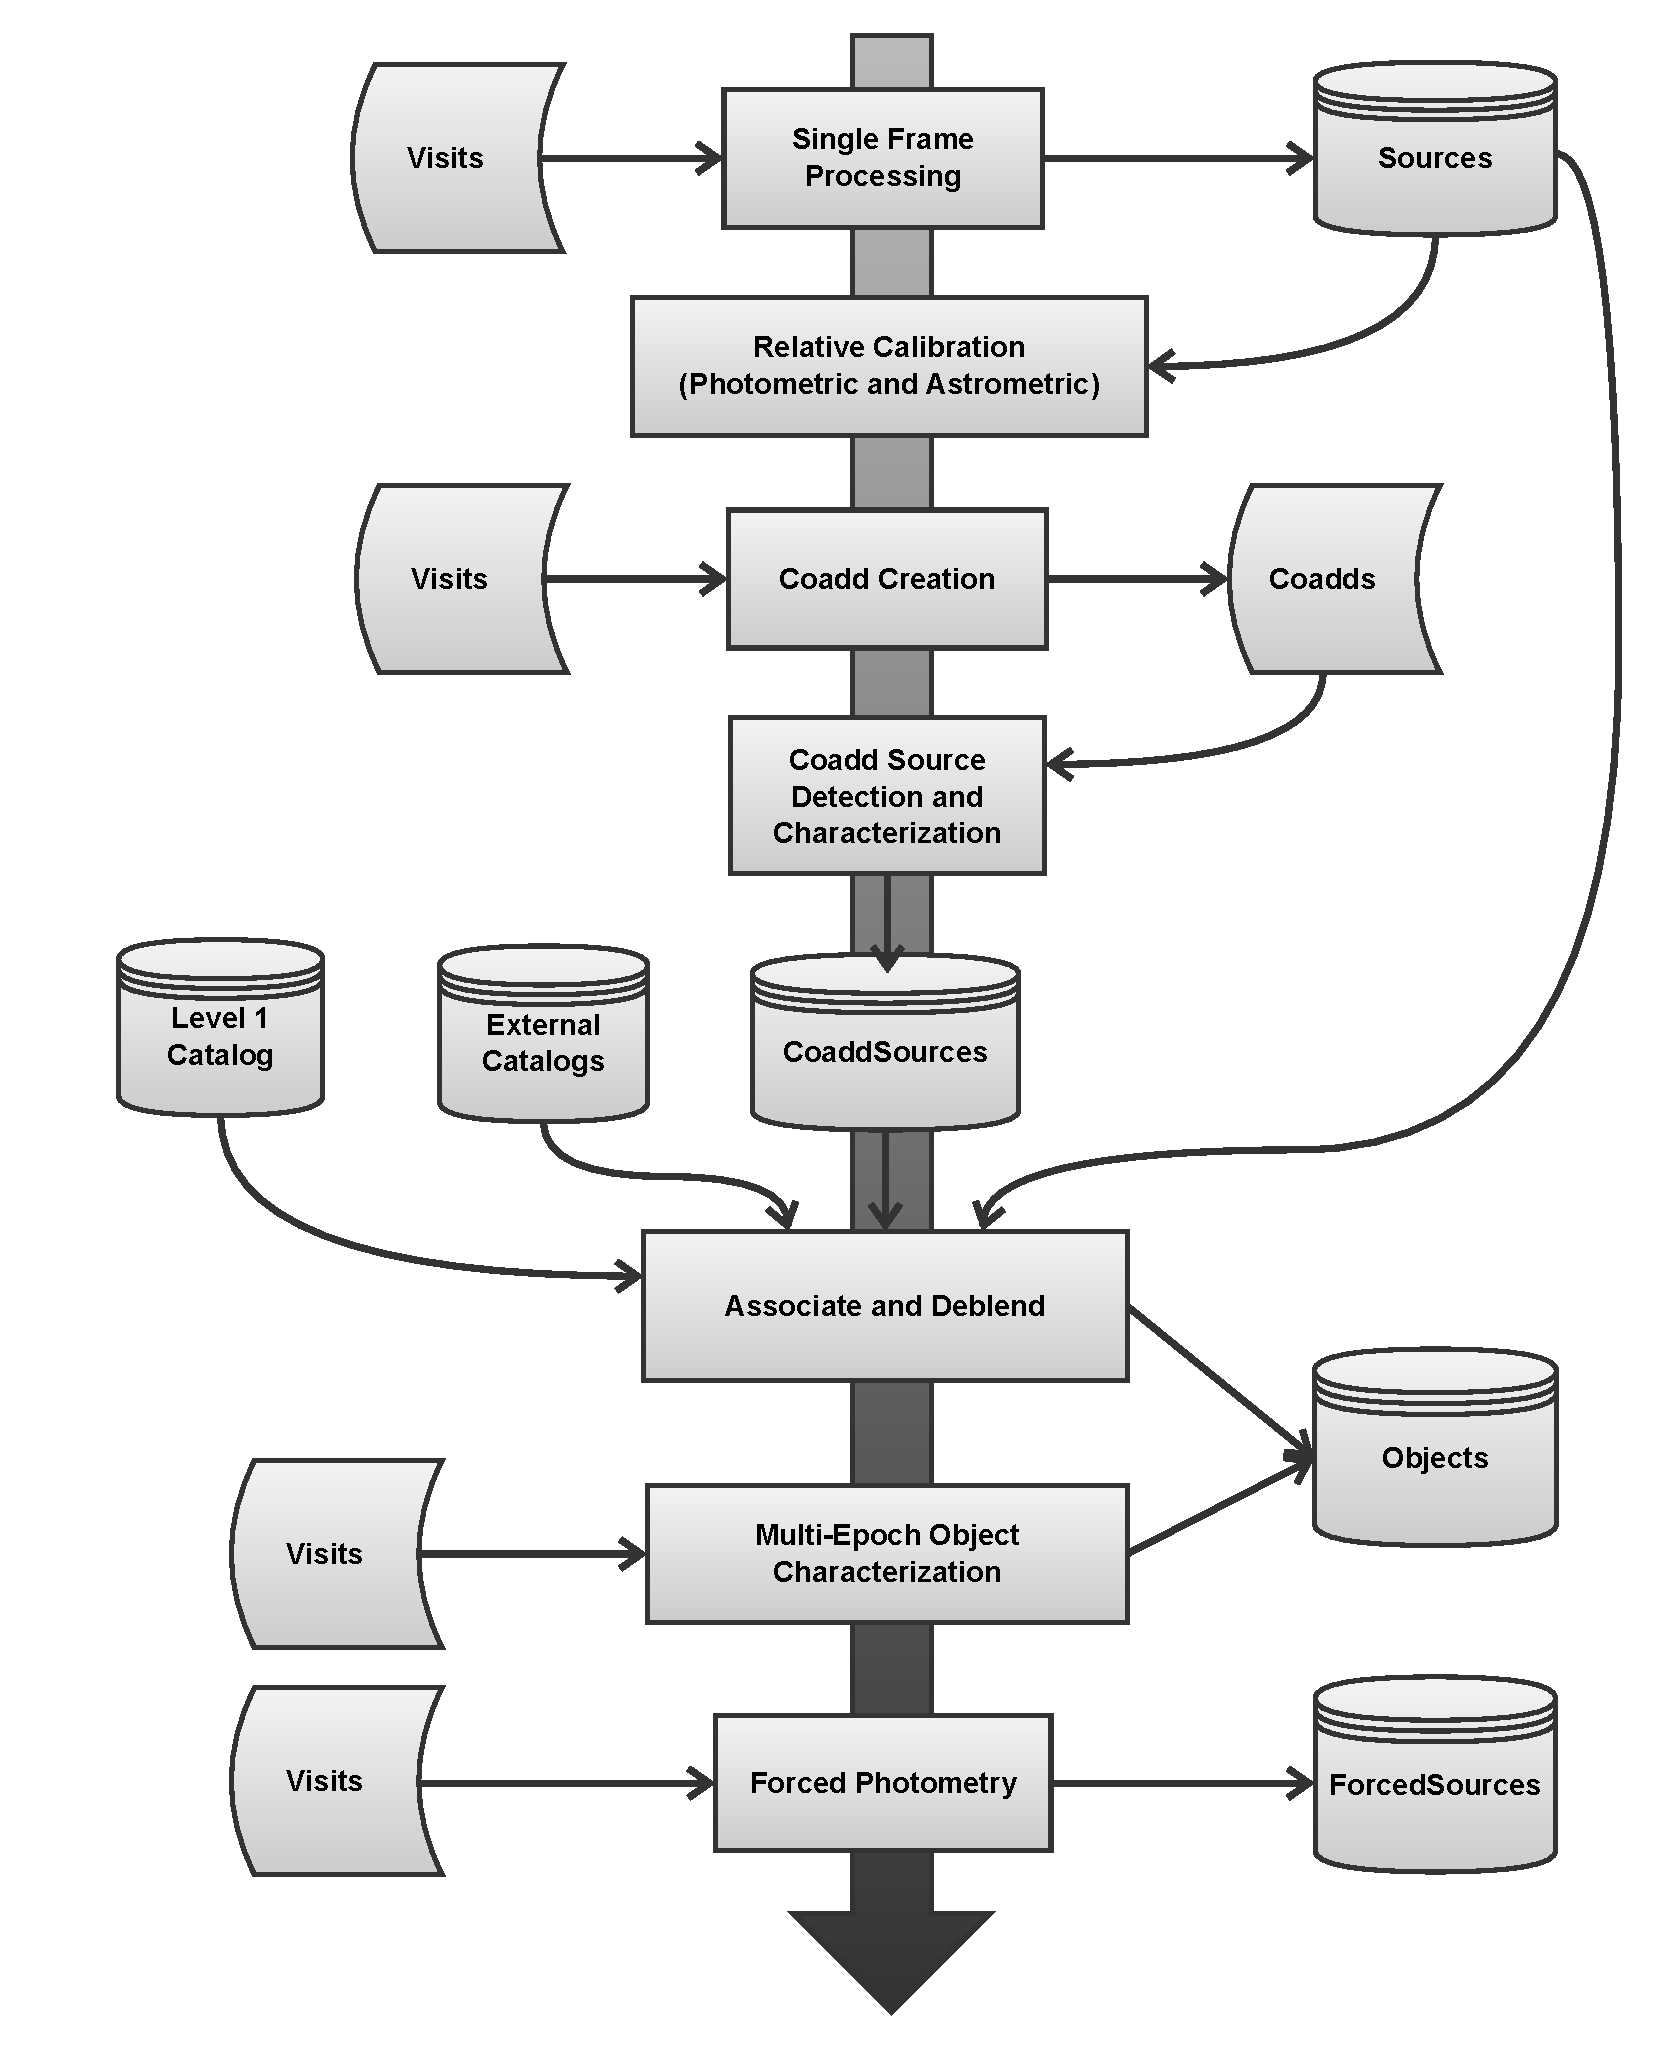
\includegraphics[scale=0.5]{figures/Level_2_Processing_Flowchart}
    \caption{Level 2 Processing Overview\label{fig:level2dp}}    
\end{figure}

Figure~\ref{fig:level2dp} presents a high-level overview of the Level 2 data processing workflow. Logically\footnote{The actual implementation may parallelize these steps to the extent possible; see LDM-230, the Automated DM Operations Document (\DMOps).}, the processing begins with single-frame (visit) image reduction and source measurement, followed by global astrometric and photometric calibration, coadd creation, detection on coadds, association and deblending, object characterization, and forced photometry measurements. The UML Use Case model (\appsUMLusecase) captures these activities in the \uc{Produce a Data Release} diagram.
\\

The following is a high-level description of steps which occur during regular Level 2 data processing:
\begin{enumerate}
    \item \emph{Single Frame Processing}: Raw exposures are reduced to \emph{calibrated visit exposures}, and \Sources are independently detected, deblended, and measured on all visits. Their measurements (instrumental fluxes and shapes) are stored in the \Source table. This step is performed by the {\bf \emph{Single Frame Processing Pipeline}} (\wbsSFM).
    \item \emph{Relative calibration}: The survey is internally calibrated, both photometrically and astrometrically using the {\bf \emph{Astrometric}} (\wbsAstroCal) and {\bf \emph{Photometric Calibration Pipelines}} (\wbsPhotoCal). Relative zero points over the focal plane and astrometric corrections are computed for every visit.
    \item \emph{Coadd creation}: Deep, seeing optimized, and short-period per-band coadds are created in $ugrizy$ bands, as well as deeper, multi-color, coadds. This task is performed by the {\bf \emph{Image Coaddition Pipeline}} (\wbsCoadd). Transient sources (including Solar System objects, explosive transients, etc), will be rejected from the coadds.
    \item \emph{Coadd source detection}. Sources will be detected on all coadds generated in the previous step. The source detection algorithm will detect regions of connected pixels, known as \emph{footprints}, above the nominal $S/N$ threshold in the \emph{PSF-likelihood image} of the visit. Each footprint may have one or more \emph{peaks}, and the collection of these peaks (and their membership in the footprints) are the output of this stage. This information will be stored in a catalog of \CoaddSources. The detection is performed by the {\bf \emph{Object Detection and Deblending}} system (\wbsDetDeblend).
    \item \emph{Coadd source deblending and characterization}. The next stage in the pipeline will decompose the \CoaddSources into a set of individual astronomical sources which is consistent across all bands, a process known as \emph{deblending}. The deblender may make use of the catalogs of \Sources and \CoaddSources, catalogs of \DIASources, \DIAObjects and \SSObjects detected on difference images, and objects from external catalogs. The deblended objects will then be characterized by measuring their positions, shapes and fluxes on the coadded images and by fitting galaxy models. This functionality is contained within the {\bf \emph{Object Detection and Deblending}} system (\wbsDetDeblend) and the {\bf \emph{Object Characterization Pipeline}} (\wbsObjChar).
    \item \emph{Multi-epoch object characterization}. A set of measurements (including predefined classes of model fits) will be performed on each of the \Objects identified in the previous step, taking all available multi-epoch data into account. Model fits will be performed using \emph{MultiFit}-type algorithms. Rather than coadding a set of images and measuring object characteristics on the coadd, MultiFit simultaneously fits PSF-convolved models to the objects multiple observations. This reduces systematic errors, improves the overall $S/N$, and allows for fitting of time-dependent quantities degenerate with shape on the coadds (for example, the proper motion). The models we plan to fit will \emph{not} allow for flux variability. Object characterization is a part of the {\bf \emph{Object Characterization Pipeline}} (\wbsObjChar).
    \item \emph{Forced Photometry}. Source fluxes will be measured on every visit, with the position, motion, structural parameters, and deblending characterized in the previous step kept fixed.
      % RHL we're not clear about which model we'll use for this forced photometry. The best-fit Sersic? 
      This process of \emph{forced photometry}, will result in the characterization of the light-curve for each object in the survey. Forced photometry is functionally a part of the {\bf \emph{Object Characterization Pipeline}} (\wbsObjChar).
\end{enumerate}


% \subsubsection{Calibration Pipelines}

\subsubsection{Enabling Level 3 Pipelines}

Level 3 capabilities are envisioned to enable science cases requiring further custom user-specified processing, especially the kind that would greatly benefit from co-location within the LSST Data Access Center. The high-level requirement for Level 3 is established in \S 3.5 of the LSST SRD.

To enable Level 3 use cases, LSST Data Management pipelines will be designed in a modular fashion to maximize the potential for reusability and synergy between Level 3 and Levels 1 and 2.

For example, a typical Level 3 use case will be to perform a different kind of measurement on objects detected in the course of Level 2 processing. A user will be able to do this by reusing the desired components of Level 2 processing, plugging in (via Python {\tt import} directives in the appropriate configuration file) the modules for their custom measurement, and executing the pipeline. The {\bf \emph{Science Pipeline Toolkit}} (\wbsSPT) will provide the necessary components to support user-driven construction and execution of custom pipelines.

\subsubsection{Science Data Quality Analysis Pipeline and Toolkit}

Science Data Quality Analysis requirements are described in the Data Quality Assurance Plan (\SDQAP) document. They will be implemented by the {\bf \emph{SDQA Pipeline}} (\wbsSDQAP; the data collection backend) and the {\bf \emph{SDQA Toolkit}} (\wbsSDQAT; the data analysis front-end).
\\

LSST QA will include four main components, which to some extent reflect the Level 1-3 structure of LSST data products. Level 0 QA is software development related, Level 1 QA relates to nightly operations, Level 2 QA relates to data releases, and Level 3 QA is science based.

\begin{itemize}
    \item {\bf Level 0 QA} includes the extensive and thorough testing of the DM subsystem during the pre-commissioning phase, as well as the tests of software improvements during the commissioning and operations phases (regression tests based on pipeline outputs and input truth). A common feature of Level 0 QA is the use of LSST simulations products, or any other dataset where the truth is sufficiently well known (e.g., the use of high-resolution observations from space telescopes to test resolved/unresolved object separation algorithms). The main goal of Level 0 QA is to quantify the software performance against these known expected outputs (e.g., to measure the completeness and false positive rate for an object finder; to measure the impact of blended sources on pipeline outputs; to measure the performance of calibration pipelines and MOPS), and to test for algorithm implementation problems (a.k.a. “coding bugs”).
    
    \item {\bf Level 1 QA} assesses the system status and data quality in real time during commissioning and operations. Its main difference from other observatory, telescope, and camera status reporting tools will be heavy reliance on the massive science imaging data stream (in addition to various telemetry and metadata generated by the subsystems). This level is tasked with nightly reporting of the overall data quality, including the nightly data products (difference images and transient source event stream) and calibration products. Real-time information about observing conditions, such as sky brightness, transparency, seeing, and about the system performance, such as the achieved faint limit, will be delivered by Level 1 QA\@. Because the actual science data stream will be analyzed, Level 1 QA tools will be in a good position to discover and characterize subtle deterioration in system performance that might not be easily caught by tools employed by the telescope and the camera subsystems for self-reporting purposes.

    \item {\bf Level 2 QA} assesses the quality of data products scheduled for the Data Releases, and provides quantitative details about data quality for each release (including the co-added image data products, and the properties of astrometrically and photometrically variable objects). This level also performs quality assessment for astrometric and photometric calibration, as well as for derived products, such as photometric redshifts for galaxies
      % RHL are we responsible for photo-z quality?  I thought it was Level 3
      and various photometric estimators for stars. Subtle problems with the image processing pipelines and systematic problems with the instrument will be discovered with Level 2 QA.
    
    \item {\bf Level 3 QA} quality assessment will be based on science analysis performed by the LSST user community. LSST will not develop Level 3 QA tools, but Level 0-2 visualization and data exploration tools will be made available to the community to form a basis on which Level 3 tools can be built. Common features expected for tools at this level are sensitivity to subtle systematic issues not recognized by Level 2 QA, and feedback about data quality to the project by external teams. It is envisioned that especially useful Level 3 QA tools would be migrated to Level 2 QA.

\end{itemize}
